\documentclass[
	12pt,				% tamanho da fonte
	oneside,			% para impressão em recto e verso. Oposto a oneside
	a4paper,			% tamanho do papel. 
	english,			% idioma adicional para hifenização
	brazil,				% o último idioma é o principal do documento
	]{abntex2}

% ---
% Pacotes fundamentais 
% ---
\usepackage{lmodern}			% Usa a fonte Latin Modern
\usepackage[T1]{fontenc}		% Selecao de codigos de fonte.
\usepackage[utf8]{inputenc}		% Codificacao do documento (conversão automática dos acentos)
\usepackage{indentfirst}		% Indenta o primeiro parágrafo de cada seção.
\usepackage{color}				% Controle das cores
\usepackage{graphicx}			% Inclusão de gráficos
\usepackage{microtype} 			% para melhorias de justificação
\usepackage{multicol}
\usepackage{multirow}
\usepackage[brazilian,hyperpageref]{backref}	 % Paginas com as citações na bibl
\usepackage[alf]{abntex2cite}	% Citações padrão ABNT
\usepackage{float}
% --- 
% CONFIGURAÇÕES DE PACOTES
% --- 

% ---
% Configurações do pacote backref
% Usado sem a opção hyperpageref de backref
\renewcommand{\backrefpagesname}{Citado na(s) página(s):~}
% Texto padrão antes do número das páginas
\renewcommand{\backref}{}
% Define os textos da citação
\renewcommand*{\backrefalt}[4]{
	\ifcase #1 %
		Nenhuma citação no texto.%
	\or
		Citado na página #2.%
	\else
		Citado #1 vezes nas páginas #2.%
	\fi}%
% ---

% ---
% Informações de dados para CAPA e FOLHA DE ROSTO
% ---
    \titulo{Prática 16: Matrizes Esparsas usando Dicionários/Conjuntos\\Laboratório de Algoritmos e Estrutura de Dados}
\autor{Pedro Inácio Rodrigues Pontes}
\local{Belo Horizonte, Brasil}
\data{2024}
\instituicao{%
  Universidade Federal de Minas Gerais
  \par
  Colégio Técnico
  \par
  Curso Técnico em Desenvolvimento de Sistemas}

\definecolor{blue}{RGB}{41,5,195}

\makeatletter
\hypersetup{
     	%pagebackref=true,
		pdftitle={\@title}, 
		pdfauthor={\@author},
    	pdfsubject={\imprimirpreambulo},
		colorlinks=true,       		% false: boxed links; true: colored links
    	linkcolor=blue,          	% color of internal links
    	citecolor=blue,        		% color of links to bibliography
    	filecolor=magenta,      		% color of file links
		urlcolor=blue,
		bookmarksdepth=4
}
\makeatother

\renewcommand{\thesection}{\arabic{section}}
\setlength{\parindent}{1.3cm}
\setlength{\parskip}{0.2cm} 

\makeindex


\begin{document}

\selectlanguage{brazil}
\frenchspacing 

\imprimircapa

{
\ABNTEXchapterfont

\textual

% ----------------------------------------------------------
% Introdução (exemplo de capítulo sem numeração, mas presente no Sumário)
% ----------------------------------------------------------
\section{Introdução}

Foi inicialmente forncedio um código na linguagem Processing Java, o qual gerava um grafo não direcionado, com seus vértices e arestas próprios. Ele também possuía uma característica de forças de atração e repulsão entre os vertíces, além de ser sorteada uma grossura aleatória para cada aresta.

\subsection{Problema Primário}

Implementar um algoritmo para resolver o problema clássico da coloração de grafos. Nesse problema, é necessário colorir um grafo de forma que seus vértices adjacentes tenham cores diferentes e utilizando o menor número possível de cores. Até hoje não foi encontrada uma solução concreta para o problema, mas há algoritmos que são capazes de o solucionar, claramente sem alcançar a eficiência máxima que seria o uso mínimo de cores em todos os casos.

\subsection{Problemas Secundários}

Refatorar o código, trocando a matriz adjacente que representava as ligações de cada vértice com os restantes para um HashSet de PVectors (no qual PVector.x representa o vértice origem e PVector.y o vértice destino). Tal implementação leva a uma menor complexidade, já que a complexidade para encontrar um elemento em um HashSet é constante(considerando que PVector tem complexidade despresível), enquanto numa matriz adjacente é O(n).

Implementar o algoritmo de coloração de grafos antes de mostrar o grafo na tela, mostrando o grafo já com as cores selecionadas.

Usar um HashSet<Integer> para gerar cores aleatórias para a coloração do grafo

Criar um construtor que recebe o número de vértices e já cria o grafo
\subsection{Objetivos}

\begin{itemize}
    \item Consolidar o uso do HashSet, além de enteder em quais situações deve ser utilizado

    \item Enteder a lógica e uso dos algoritmos classificados como gulosos
\end{itemize}

\section{Desenvolvimento}

\subsection{Resolução da Implementação do Algoritmo Coloração de Grafos}

Para aplicar a coloração de grafos, foi utilizado o método do algoritmo guloso, que define opções classificadas como ótimas para cada subdivisão do problema. Essa metodologia foi adotada por já ter sido disponibilizada e sugerida quando o problema foi proposto pelo coordenador do curso.

Foi dado o seguinte pseudocódigo para a resolução do problema por meio do algoritmo guloso:

\begin{verbatim}
função colorirGrafo(G):
    n = número de vértices em G
    cores = array de tamanho n, inicializado com 0
    coresDisponiveis = array de tamanho n, inicializado com true

    para cada vértice v em G:
        para cada vizinho u de v:
            se cores[u] != 0:
                coresDisponiveis[cores[u]] = false

        para cor de 1 até n:
            se coresDisponiveis[cor] == true:
                cores[v] = cor
                pare

        // Resetar coresDisponiveis para o próximo vértice
        para i de 1 até n:
            coresDisponiveis[i] = true

    retornar cores
\end{verbatim}

Abaixo, código real, em Processing Java, gerado a partir dele:

\begin{verbatim}
int[] colorirGrafo() {
   int n = numVertices;
   int cores[] = new int[n];
   boolean coresDisponiveis[] = new boolean[n];
   HashSet<Integer> coresUtilizadas = new HashSet<Integer>();

   for (int i = 0; i < n; i ++) {
     cores[i] = 0;
     coresDisponiveis[i] = true;
   }

   for (int v = 0; v < n; v ++) {
     for (int u = 0; u < n; u ++) {
       if (cores[u] != 0 && arestas.containsKey(new PVector(v, u))) {
         coresDisponiveis[cores[u]] = false;
       }
     }


     for (int cor = 1; cor < n; cor++) {
       if (coresDisponiveis[cor] == true) {
         cores[v] = cor;
         break;
       }
     }

     for (int i = 1; i < n; i ++) {
       coresDisponiveis[i] = true;
     }
   }

   while (coresUtilizadas.size() <= cores.length) {
     int corReal = color(random(0, 255), random(0, 255), random(0, 255));
     coresUtilizadas.add(corReal);
   }
   coresReais = new ArrayList<Integer>(coresUtilizadas);
   return cores;
}    
\end{verbatim}

Aqui, faz-se o alarde de que o \textit{while}, a atribuição a \textit{coresReais}, logo abaixo dele, e a declaração do \textit{HashSet CoresUtilizadas}, não fazem parte da tradução desse pseudocódigo, pertecendo à parte física da coloração em si do grafo.

O código verifica se uma cor está disponível para um vértice a partir do preceito que seus vizinhos não a utilizam. No fim, ela utiliza como solução ideal, para o subproblema da coloração de cada vértice, o vértice vizinho ter uma cor. A partir disso, ela marca a cor disponível como falsa para o vértice tomado como referência. Após isso, há outro subproblema em que a solução ideal vem de quando a cor está disponível, daí, é colocada no indíce referente ao vértice. Em resumo, verifica se o vértice vizinho possui certa cor, se possuir, marca ela como falsa, e vai iterando sobre todas as cores existentes. Se nenhuma delas estiver disponível, cria outra.

\subsection{Solução da Coloração do Grafo}

A partir do algoritmo da coloração do grafo, é retornado um array \textit{cores} que contém o número da cor que cada vértice deve ter, ex: \textit{cores[vértice A] = 1}. A questão agora, é fazer tal resultado refletir no código palpável, pois o valor retornado não estava sendo utilizado para nada. Esse caso foi dividido em dois problemas: Gerar cores aleatórias para representarem cada número possível de ser retornado no array \textit{cores} e aplicar isso à função desenhar.

\subsubsection{Cores Aleatórias}
Para gerar cores reais a partir dos números retornados pelo array, foi criado, como pedido, um \textit{HashSet}, nomeado como coresUtilizadas. Tal implementação leva à impossibilidade de haverem duas cores repetidas, evitando um problema de ser atribuída a mesma cor a retornos diferentes de \textit{cores}. Para preencher esse HashSet de cores aleatórias, foi utilizado o seguinte while, implementado no fim da função colorir grafo (a qual implementa o algoritmo de coloração):

\begin{verbatim}
 while (coresUtilizadas.size() <= cores.length) {
  int corReal = color(random(0, 255), random(0, 255), random(0, 255));
  coresUtilizadas.add(corReal);
}
\end{verbatim}

Perceba que o uso do while dentro da função \textit{colorirGrafo} gera a impossiblidade desta ser chamada mais de uma vez para o mesmo grafo, pois geraria novas cores aleatórias. Isso não afeta em nada no programa, e auxilia na tarefa de já definir as cores antes de desenhar o grafo, pois \textit{colorirGrafo} não poderia ser chamada dentro de desenhar, pois tal é chamada em um loop infinito dentro da função \textit{draw}. 

Após serem adicionadas essas cores, é necessário relacioná-las cada uma com um possível retorno de \textit{cores}, para isso, foi criada uma ArrayList com base em \textit{CoresUtilizadas}: \textit{coresReais = new ArrayList<Integer>(coresUtilizadas);}. Ela foi declarada como um atributo da classe grafo, para poder ser acessada livremente dentro da classe. Isso será importante na parte de implementar o código em \textit{desenhar()}.

\subsubsection{Coloração Efetiva}

Para a coloração ocorrer efetivamente, a função \textit{desenhar} teve de ser atualizada dentro do \textit{fill()} que definia a cor de cada vértice (inicialmente ele sempre era definido como branco, 255). Essa atualização foi feita utilizando-se \textit{fill(coresReais.get(cores[arestaOrigem]));}. É utilizada a cor relativa ao indíce que representa o vértice em questão. 

\textit{cores[arestaOrigem]}: é a cor númerica/falsa para a aresta em questão.

\textit{coresReais.get}: Obtém a cor real na ArrayList coresReais a partir do índice fornecido por \textit{cores[arestaOrigem]}.

\subsection{Refatoramento}

O refatoramento foi feito a partir da troca dos métodos de acesso e inserção de uma matriz adjacente pelos de um HashMap, mais os parâmetros do PVector. Não foi utilizado o HashSet pela questão de, no código original, aresta ter um valor de grossura, armazenado na matriz adjacente. Para manter esse comportamento, foi necessário usar um HashMap, onde a chave é o PVector que guarda os vértices origem e destino da aresta, e o valor é a grossura da aresta.

As mudanças principais são normalmente dos seguintes tipos ou variações deles:
\begin{verbatim}
matrizAdj[i][j] = 2    para    arestas.put(new PVector(i,j), 2)


for(int i = 0; i < numVetices; i ++){
    for(int j = 0; j < numVertices){
    
    }
}   

para

for(PVector aresta: arestas.keySet()){}} (i fica igual aresta.x e j, aresta.y)
\end{verbatim}

A função que melhor representa a refatoração é \textit{desenhar()}:

Antes:


\begin{verbatim}
void desenhar() {
   textAlign(CENTER);
   // Desenha as arestas
   stroke(0);
   strokeWeight(1);
   for (int i = 0; i < numVertices; i++) {
       for (int j = i + 1; j < numVertices; j++) {
           strokeWeight(matrizAdj[i][j]);
           if (matrizAdj[i][j] > 0) line(posicoes[i].x, posicoes[i].y, posicoes[j].x, posicoes[j].y);
       }
   }

   // Desenha os nós
   fill(255);
   stroke(0);
   strokeWeight(1);
   for (int i = 0; i < numVertices; i++) {
       fill(255);
       ellipse(posicoes[i].x, posicoes[i].y, raio * 2, raio * 2);
       fill(0);
       text(str(i), posicoes[i].x, posicoes[i].y+4);
   }
}
\end{verbatim}


Depois:


\begin{verbatim}
void desenhar(int[] cores) {
  textAlign(CENTER);
  // Desenha as arestas
  strokeWeight(1);
  for (Map.Entry<PVector, Integer> aresta : arestas.entrySet()) {
    int arestaOrigem = (int) aresta.getKey().x;
    int arestaDestino = (int) aresta.getKey().y;
    stroke(0);
    strokeWeight(aresta.getValue());
    if (aresta.getValue() > 0) line(posicoes[arestaOrigem].x, posicoes[arestaOrigem].y, posicoes[arestaDestino].x, posicoes[arestaDestino].y);
  }

  // Desenha os nós
  fill(255);
  strokeWeight(1);
  for (PVector aresta : arestas.keySet()) {
    int arestaOrigem = (int) aresta.x;
    fill(coresReais.get(cores[arestaOrigem]));
    ellipse(posicoes[arestaOrigem].x, posicoes[arestaOrigem].y, raio * 2, raio * 2);
    fill(0);
    text(str(arestaOrigem), posicoes[arestaOrigem].x, posicoes[arestaOrigem].y+4);
  }
}
\end{verbatim}

Perceba a diferença na estrutura dos laços \textit{for}, em como é utilizado o código para obter o valor de cada vértice e seu adjacente e para obter a grossura de cada aresta. Note a melhora na legibilidade do código.

\subsection{Construtor com Número de Vértices}

Foi adicionado o código:

\begin{verbatim}
Grafo(int numVertices) {
  int[][] adj = new int[numVertices][numVertices];

  for (int i = 0; i < numVertices; i++)
    for (int j = 0; j < numVertices; j++) {
      if (i == j) {
        adj[i][j] = 0;
      } else {
        if (random(1) > 0.5) {
          arestas.put(new PVector(i, j), (int) random(1, 5)) ;
          arestas.put(new PVector(j, i), arestas.get(new PVector(i, j)));
        }
      }
    }
  this.numVertices = numVertices;
  posicoes = new PVector[numVertices];
  velocidades = new PVector[numVertices];
  inicializarPosicoes();
}
\end{verbatim}
\section{Resultados}
\begin{figure}[H]
\centering
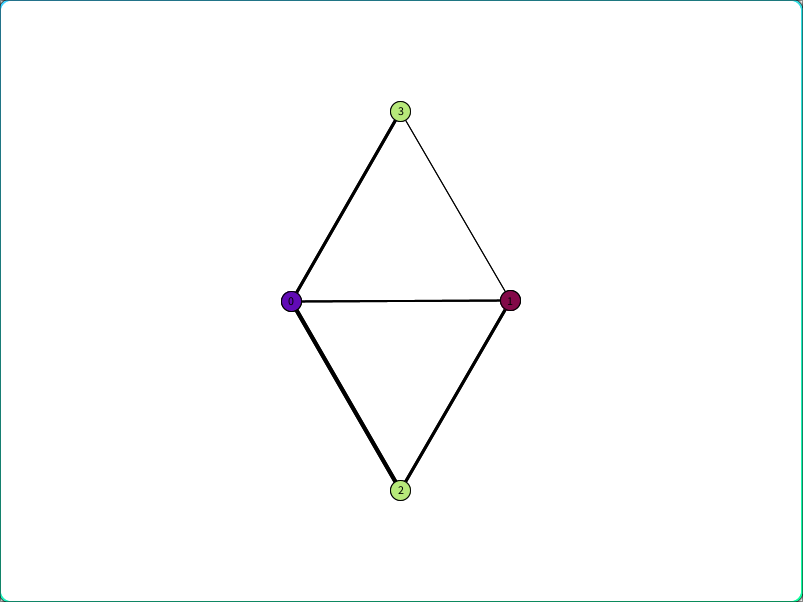
\includegraphics[width=0.9\textwidth]{imgs/img1.png}
\label{imagem 0.9}
\end{figure}
\begin{figure}[H]
\centering
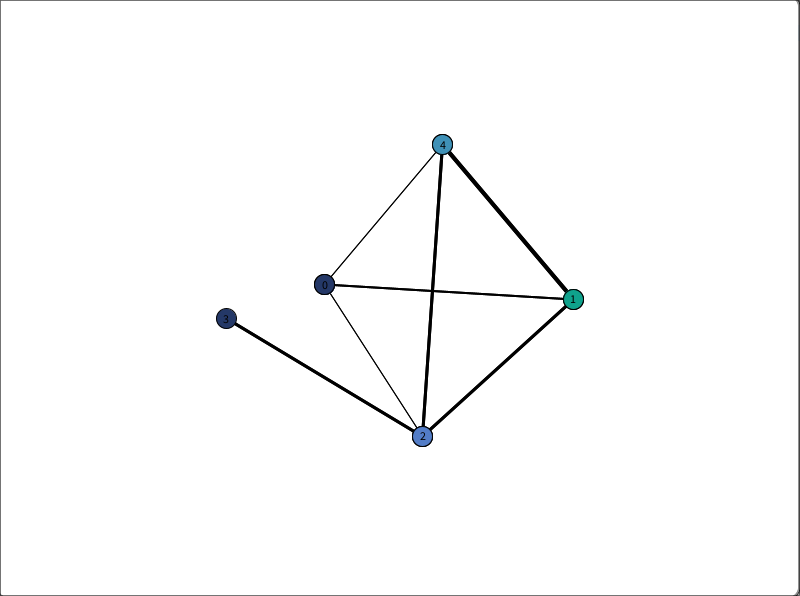
\includegraphics[width=0.9\textwidth]{imgs/img2.png}
\label{imagem 2}
\end{figure}
\begin{figure}[H]
\centering
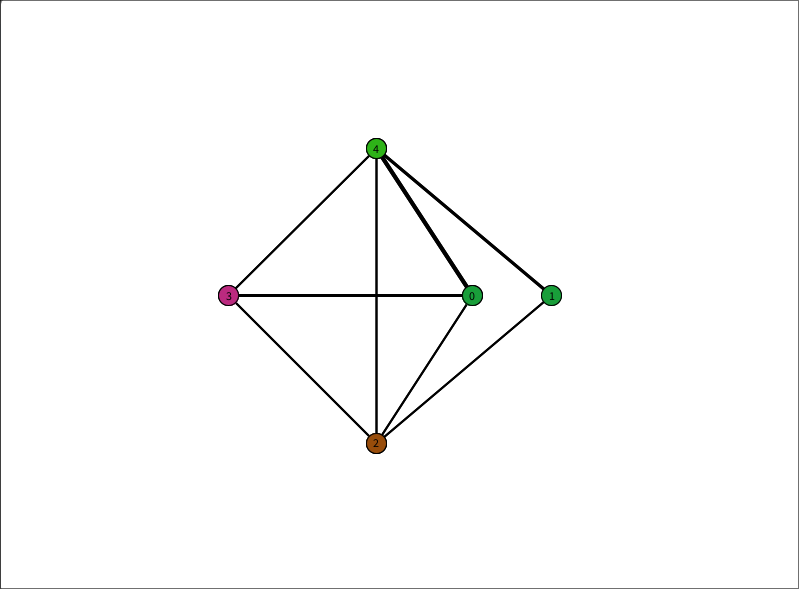
\includegraphics[width=0.9\textwidth]{imgs/img3.png}
\label{imagem 3}
\end{figure}
\begin{figure}[H]
\centering
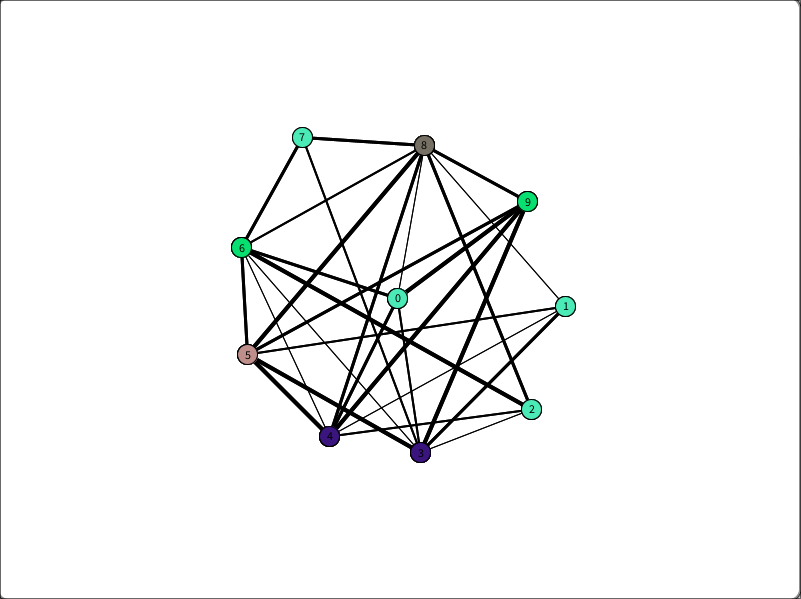
\includegraphics[width=0.9\textwidth]{imgs/img4.png}
\label{imagem 4}
\end{figure}
\begin{figure}[H]
\centering
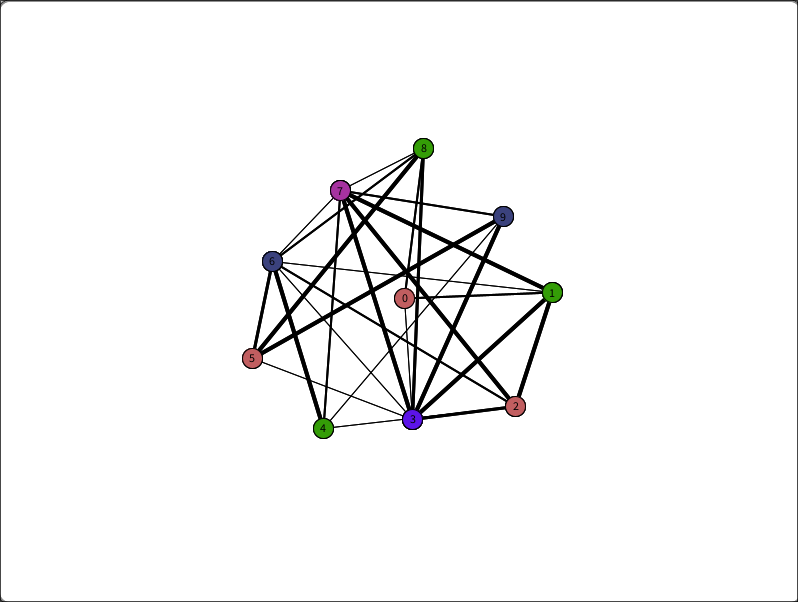
\includegraphics[width=0.9\textwidth]{imgs/img5.png}
\label{imagem 5}
\end{figure}

\section{Conclusão}

Os resultados encontrados estão totalmente de acordo com o objetivo, aplicando-se o algorito de coloração de grafos e entendo como ele funciona e suas falhas. Além disso, houve o entendimento do algoritmo guloso em sua teoria. O desvio mais significativo dos objetivos foi o uso de um HashMap<PVector, Integer> para guardar as arestas. Isso foi feito unicamente para guardar o valor da grossura de cada aresta, e não apresentou nenhuma consequência negativa para o código, no fim, só foi um exercício da capacidade crítica da melhor escolha para cada situação.

As principais dificuldades do experimento foram a adaptação do algoritmo guloso do pseudocódigo para o código usando o HashMap de PVectors guardando as arestas, a lógica do algoritmo foi incrivelmente difícil de aplicar, e houve uma grande dificuldade por a estrutura inicial estar errada, assim, as horas de tentativas de mudança para corrigí-lo foram em vão, pois o problema era estrutural. Entender como aplicar o algoritmo \textit{colorirGrafo} efetivamente no código também foi uma dificuldade grande, pois para isso é necessária um entendimento completo do código seus resultados esperados e reais, além das deficiências dele, junto de uma capacidade enorme de abstração. Por fim, a última dificuldade foi o tempo consumido para fazer todo o necessário, mais de 12 horas no total.

\end{document}
